%!TEX root = geovis-boilerplate.tex


\begin{abstract}
This paper presents extensions to the Imperfect Shadow Map algorithm used to compute visibility for many-light global illumination methods. The extensions combine compute shaders for rendering with an advanced postprocessing algorithm for surface reconstruction to improve the quality of the shadowmaps. This goal is achieved at the expense of performance and memory requirements, but at the same time comes with better scalability with regards to the captured geometric detail.
\end{abstract}



\section{Introduction}
For decades, computer graphics researchers have strived to achieve the faithful reproduction of reality in synthetic renderings. While photorealism has been achieved in offline rendering contexts, many optical effects occurring in physical environments are still not in use in interactive and real-time applications or implemented with severe limitations. Several lighting effects collectively referred to as ``global illumination'', such as caustics, subsurface scattering and diffuse and specular indirect light, fall into this category.

Many-light methods are one class of algorithms that has been used to simulate such effects. They use masses of \textit{Virtual Point Lights} (VPLs) placed in the scene to simulate reflected and refracted light. While the simulation of more advanced effects requires a large amount of lights (hundreds of thousands to millions) and is thus limited to offline rendering, it is possible to create a fairly accurate indirect lighting effect in real-time with only a few thousand lights.

A major problem when simulating indirect lighting with many-light methods is to compute visibility between the VPLs and the scene. While conventional shadow maps can be used, they are generally too slow to be re-computed every frame for every VPL. To this end, \textit{Imperfect Shadow Maps} (ISMs) have been proposed, an approximated form of shadow maps. They convert the scene's geometry to points and render those to thousands of small shadow maps.

In this paper, we propose an extension to ISMs that enables more complex scenes to be captured more accurately. On the one hand, we use a more advanced postprocessing method for reconstructing the scene's surfaces. On the other hand, we make use of compute shaders to provide better scalability when rendering large amounts of points, further contributing to higher accuracy.




\section{Related Work}

Many-light methods for simulating global illumination effects are a well-researched topic. They are based on Instant Radiosity \cite{Keller:1997:InstantRadiosity}, which uses a process similar to photon mapping to trace rays through the scene, but instead of storing intersections as photon in a photon map, it creates a new VPL per intersection. The VPLs are then used to illuminate the scene.

The two major problems that need to be solved when building a many-light rendering system are VPL placement and solving occlusion. A third problem, mitigating singularities, is very easily solved when accepting bias in the rendering.


The foundation of many algorithms for VPL placement are \textit{Reflective Shadow Maps} (RSMs) \cite{Dachsbacher:2005:RSM}, which are shadow maps with additional surface information. Using the additional data, VPLs are created per texel of the RSM. View-adaptive placement of VPLs greatly enhances performance and quality \cite{ritschel2011ismsViewAdaptive}. RSM samples can be clustered to form virtual area lights \cite{prutkin2012reflective}, and \cite{hedman2016sequential} focus on temporal coherence when placing VPLs to avoid flickering.

A common approach for solving occlusion are Imperfect Sha\-dow Maps \cite{ritschel2008ism}, which use a point-based approximation of the scene to efficiently render a small and inaccurate shadow map for hundreds of VPLs simultaneously. ISMs have been used in production for rendering shadows for primary scene lights\cite{evans2015dreams}, and several enhancements have been proposed \cite{ritschel2011ismsViewAdaptive, hollander2011manylods, barak2013temporally}. We take several aspects of \cite{ritschel2008ism} and \cite{barak2013temporally} and propose extensions for better scalability and quality.

Other means for visibility computation can be combined with many-light methods as well. For instance, ray tracing through voxel grids has been proposed \cite{sugihara2014layered, sun2015manylightsSVO, Chen:2016:Compactvoxels}, albeit using slim voxels, i.e., using only one bit per voxel for visibility testing. This avoids the usually high memory requirements of voxelization techniques. Ray-tracing through a triangle-based scene representation is of course possible (e.\,g.\ \cite{segovia2006bidirectional}) but generally too slow to be used in a real-time context.

Singularities are an artifact of many-light methods that appear as bright spots near the VPL's positions due to the light's attenuation term approaching infinity. A common approach is to clamp the term. This introduces bias, which can be compensated e.g. in screen space \cite{novak2011screen}. Those singularities can also be avoided through more advanced light representations \cite{tokuyoshi2015vsgl}.



\section{Visibility Computation with \\ Imperfect Shadow Maps}
\label{sec:concept:ism}

Imperfect Shadow Maps \cite{ritschel2008ism} convert the scene geometry to a point set in a preprocessing step and use the points to efficiently render hundreds of shadow maps in parallel. They use splatting to render the points and fill the resulting holes in the shadow maps with a simplified version of the pull-push algorithm presented in \cite{Marroquim:2007:reconstruction}.

\cite{ritschel2011ismsViewAdaptive} build on this by converting the scene to a triangle texture dynamically, and sampling the points from that texture. Instead of computing a triangle texture, \cite{barak2013temporally} use the tessellation units of recent GPUs to dynamically convert triangles into points.
We follow this approach since it is relatively straightforward to implement and inherently dynamic, but have not implemented the adaptive sampling from \cite{ritschel2011ismsViewAdaptive} yet.
\cite{ritschel2008ism} also present multi-bounce indirect illumination with their technique, which we have not implemented.

In contrast to \cite{ritschel2008ism}, we have found the pull-push postprocessing to be of little benefit when using regular point splatting. Instead, we propose to render the points as single pixels, which opens interesting optimization opportunities, but in turn requires the pull-push algorithm to reconstruct the scene surfaces.

We describe the regular point splat rendering process in the following section and subsequently detail the pull-push algorithm that we use when rendering single-pixel points.


\subsection{Point Rendering with Splatting}

To convert the scene into points, all its triangles are first tessellated to meet a certain maximum size in order for the point conversion to not introduce extreme inaccuracies. Of the smaller tessellated triangles, the center and area are calulated and a point with matching center and area is created. While it might be more performant to create points just on the vertices of the triangles, at the same time it will be more inaccurate since this approach will enlarge the rendered area considerably over the triangle's extents.

Now a random VPL is chosen per point and backface culling is performed. Likewise, points that lie behind their VPL's illuminated hemisphere are culled before splatting the point into the respective ISM. For performance reasons, a simple paraboloid projection is used for the ISMs in lieu of conventional cubemaps. Here, another advantage of using points comes into play: Compared to triangles, it is trivial to perform a paraboloid projection on them.

As an optimization, we iterate over several VPLs per point, collect those that pass the culling test and render to all the collected ones. More on this in \Cref{sec:impl:singlePixelRendering}.

To remove holes in the resulting shadow map, the original paper implements a simplified variant of \cite{Marroquim:2007:reconstruction} that only uses depth information from the point rendering. We found that this approach has little benefit over simply enlarging all the point splats during rendering, therefore we did not use it when using splat rendering.



\subsection{Point Rendering with Pull-Push Postprocessing}

As an alternative to point splat rendering, this subsection proposes a second approach that follows the algorithm of \cite{Marroquim:2007:reconstruction} more closely with the intent to obtain higher-quality shadow maps. More specifically, the points are rendered as a single pixel, albeit with additional attributes like size and normal. These are then used in a subsequent reconstruction pass to create an (ideally) hole-free shadow map. This approach also allows a point to be rendered into multiple shadow maps with a moderate performance impact, more on this in \Cref{sec:impl:singlePixelRendering}.

To provide a rough overview, the pull-push algorithm proposed by \cite{Marroquim:2007:reconstruction} is a ``pyramid-method'' (see \cite{Strengert:2006:Pyramid}) that uses the mipmap levels of a texture to first condense and then spread the data in the texture, in this case the sparse point set representing the scene. During the pull phase, it aggregates the information from four pixels of a finer level to one pixel of a coarser level. The subsequent push phase aggregates four pixels of a coarser level to one pixel of a finer level, but only if the pixel of the finer level contains no data or is determined to belong to an occluded surface. This way, closed surfaces are derived from single-pixel points.

\subsubsection{Pull Phase}
The pull phase reads four pixels of a finer level, computes an aggregate representation of them and writes the result to one pixel of the next coarser level. However, it only considers pixels that pass the following tests: First, they need to contain a valid depth at all (i.\,e., a point must have been rendered into this pixel) and second, the point in this pixel must not be occluded. A point is considered to be occluded if it is outside  the depth interval of the frontmost of the four pixels used for interpolation.

Figuratively speaking, the depth interval of a point denotes the range in which other points are considered to belong to the same surface and can be used for interpolation. For the rendered points, the depth interval is simply $[d;d+k]$ where $d$ is the points depth and $k$ an arbitrarily chosen constant. For interpolated points, the new depth interval spans the interpolated depth of the point to the highest depth value of the depth intervals of all ``parent'' points.

To calculate the attributes for a new point, the depth and radius of the parent points are interpolated in between with equal weights. Since the center of the aggregated point might not match with the position of the pixel (this happens if not all four pixels are used for interpolation), a displacement vector is also calculated and stored to accurately describe the point's location.


\subsubsection{Push Phase}

Analogous to the pull phase, the push phase reads four pixels of the coarser level, rejects pixels that don't pass certain tests, and writes one output pixel into the finer level. First, just like in the pull phase, the input pixels must contain a valid depth and not be occluded to be considered. Additionally, a radius check is performed: If the pixel's location is outside the point's extents described by the displacement vector and its radius, then the point is not considered either. This is done to limit a point's influence to its actual size.

The target output location in the finer level might already contain data computed during the pull phase. This data is overwritten if its depth is behind the interpolated point's depth interval, i.e. if the original data is considered to be occluded. Otherwise, the original point is left untouched, as it is likely more accurate than the just computed, interpolated point.

Since the input and output pixel's location do not match the way they do during the pull phase, the weights used for interpolation during the push phase are not uniform.

 \cite{Marroquim:2007:reconstruction} also use the point's normals to correctly limit the point's size, and \cite{Marroquim:2008:reconstruction2} propose gaussian weights based on the pixel's distance to the point's location, instead of constant weights solely based on pixel locations. Both of these additions we have not implemented yet.







 \section{Implementation}
 \label{sec:impl}

The ISM algorithm is embedded in a larger system for computing indirect lighting in real-time. The system uses reflective shadow maps \cite{Dachsbacher:2005:RSM} that are regularly sampled to create VPLs. The ISMs are rendered each frame right after the VPLs have been sampled.

 \subsection{Point Creation}
 \label{sec:impl:pointCreation}

 Both the point splat renderer and the single-pixel point renderer share the first stages of their rendering pipelines, which are described here, before the following subsections describe the two renderers themselves and the pull-push postprocessing.

 We make use of OpenGL's tessellation shader to subdivide triangles to make them meet a certain maximum size. The tessellation control shader determines the tessellation levels according to the triangle's size. The tessellation evaluation shader does nothing more than correctly interpolating the vertex positions.

 The geometry shader, which now recieves the smaller, tessellated triangles, converts each triangle to a point. The point's center equals the triangle's center, and the radius is chosen so the areas of the point and triangle match.

 While a random subset of all points needs to be chosen for each ISM, special care must be taken to make sure that the same subset of points is used for each ISM in each frame. Otherwise, the ISMs will be temporally incoherent and cause flickering in the final rendering. To this end, the point's barycentric coordinate inside its triangle and the triangle's \texttt{gl\_PrimitiveID} are passed to a fast hashing algorithm. The result is is used to determine an ISM ID (or, equivalently, a VPL ID) for use in the next step.

 Note that no translation or projection has been applied yet, this happens in a later stage. As a result, the vertex shader is a simple pass-through shader.

 The next step depends on whether point splatting or the single-pixel renderer is enabled.



 \subsection{Point Rendering with Splatting}
 \label{sec:impl:splatting}

 In the case of point splatting, the geometry shader itself reads the VPL with the ID it determined, projects the point according to the VPL's data, performs culling and discards the point if necessary, sets \texttt{gl\_PointSize} to the projected size, and emits a vertex.

 The \texttt{output\_primitive} must be set to \texttt{points} in the geometry shader's \texttt{layout} definition. As explained previously, for point splatting all points are simply enlarged by a small constant factor in lieu of the pull-push postprocessing. Since only depth information are needed in this case, the fragment shader is empty.



 \subsection{Single-Pixel Point Rendering with Compute Shaders}
 \label{sec:impl:singlePixelRendering}

 This approach was inspired by the fact that the surface reconstruction in \cite{Marroquim:2007:reconstruction} works with single-pixel ``splats''. Since in this case the hardware rasterizer is not required to achieve good performance, this allowed for more flexibility and new optimization opportunities.

 The general idea is to first let the geometry shader write the generated points into a buffer, which is then used by a separate compute shader pass to perform the actual rendering.

 In order to maintain temporal coherence, the points are not written into a single large buffer, as it would be hard to consistently determine a location for each point in that buffer. Instead, the buffer is divided into one section per VPL, and the points are written into the section corresponding to the ID calculated before. An atomic counter that indicates the first free index is used per section to sequentially fill these sections without overwriting any data. The order of the points within each section is undefined, but that does not change the output since they all are going to be rendered into the same ISM.

 Now a compute shader is used to render the points. For each VPL, one work group reads through the respective section of the point buffer and performs the transformation and culling against the VPL for each point. It then uses the GLSL function \texttt{imageAtomicMin} to ``render'' the point with correct depth testing as a single pixel into the respective ISM. Since atomic operations require using single channel integer textures, it is not possible to use a second or third channel for additional attributes. Instead, the ISM is actually implemented as 3D texture, using the second index in the third dimension as additional ``render target'' to hold the radius and normal. However, this approach requires the use of 32 bit for storing the depth even if a lower precision would suffice, and the attributes need to be packed into 32-bit integers.

 As an optimization, the compute shader renders each point into several ISMs. To this end, each work group reads the data of a fixed number of VPLs (e.\,g.\ 16) into shared memory. Then, while rendering the points, the culling is performed per point on all 16 VPLs, and those VPLs where the point passes the culling test are collected into a local array. Thereafter the point is transformed for each of the collected VPLs and rendered into the respective ISM.

 % In practice it turned out to be more efficient to limit the number of slots in the local array to a constant maximum (e.\,g.\ 4), possibly because this ensures that the rendering loop is not diverging and enables compiler optimizations like loop unrolling.

 An attempt to do this optimization in the splat renderer by emitting multiple vertices in the geometry shader resulted in a significant performance hit, see \Cref{sec:results:performance}.


 \subsubsection{Race Conditions in the Single-Pixel Renderer}

 There are two race conditions that may influence the output when using the single-pixel renderer.

 First, the order of writes to the ISM depth buffer is undefined as the execution order of the different compute shaders is undefined in the OpenGL specification. Therefore, the classical z-fighting may occur if two points are rendered into the same pixel of the same shadow map with the same depth value. The attributes that end up written into the additional render target are undefined in this case and may differ between subsequent frames. In practice, this happens very rarely and we chose to ignore this.

 However, a different race condition was frequently observable in our implementation:
 If two threads with differing depth values simultaneously write into the depth buffer, using \texttt{imageAtomicMin} guarantees the correct value will end up in the buffer. However, if the higher value got written first and gets overwritten by the second write, both writes have succeeded. This results in both threads attempting to write into the second buffer, creating another race condition since the here execution order is undefined again. This problem can be alleviated by adding a synchronization point after the atomic write and then reading the memory location that just got written to. If it is equal to the written value, one can assume the write actually succeeded and did not get overwritten by a second, simultaneous write. Only then the write to the second buffer is performed.

 However, this solution fixes the race condition only inside one work group and not between work groups, for which no efficient synchronization primitives exist on the GPU. The problem occurred infrequently enough though to be negligible.

 A proper solution that would fix this problem completely, avoid the synchronization overhead and open more optimization possibilities would involve a more advanced software renderer, e.\,g.\ following the approaches of \cite{Laine:2011:SoftwareRasterization}.


 \subsection{Pull-Push Postprocessing}
 \label{sec:impl:pullPushPostprocessing}

 Our implementation of the pull-push algorithm is relatively straightforward. For each miplevel to be calculated, one \texttt{dispatchCompute} is called. Since the first step of the pull phase has different inputs than the subsequent steps (it only has depth and size, not the displacement vector and depth interval), a slightly different shader is used there. Analogous the last step of the push phase outputs only depth, therefore a shader variant is used for that step as well. For the same reason, the input texture (the ``render target'' used by the single-pixel renderer) and output texture (the final ISM used later for shadow lookups) have different formats than the mipmap levels used by the pull-push algorithm.



 In the pull phase, one compute shader invocation calculates one output pixel. It reads its four input pixels, determines which of them are valid, and uses the valid ones for interpolating.


 During the push phase, groups of four output pixels share the same input pixels. This can be exploited by letting each shader invocation compute four output pixels while still reading only four input pixels. Naturally, the weights applied to the input pixels need to be adjusted per output pixel. For invalidating input pixels, their weights can simply be set to zero instead of separately marking them as invalid.


 Note that there is still lots of room for optimization. Especially the pull phase is basically a parallel reduction which is well-researched and for which optimized algorithms on the GPU exist, see e.\,g.\ \cite{Harris:2007:ParallelReduction}. Several optimizations from that field might be applicable here.






 \section{Results}


 The implementation is tested in the Crytek Sponza scene with 260k triangles, provided by \cite{McGuire2011Data}.

 All measurements have been performed with an NVIDIA GeForce GTX 750 Ti.

 % no antialiasing but SSAO?

 Unless otherwise noted, the parameters used for the measurements and screenshots are:
 \vspace{-1em}
 \begin{itemize}
     \setlength\itemsep{0.0em}
     \item 1920x1080\,px output resolution
     \item 1024 VPLs
     \item 2048\,px\textsuperscript{2} ISM texture, i.\,e., 64\,px\textsuperscript{2} per ISM
     \item Single-pixel point renderer: 16 VPLs considered per point, up to 4 collected
 \end{itemize}


 %\Cref{fig:???} shows the Crytek Sponza scene rendered using ISMs created by the splat renderer (a) and the single-pixel renderer (b). A section of the ISM texture is shown for each renderer in the lower row.


 \subsection{Quality}

 \begin{figure}[htb]
 \centering
   \begin{tabular}{@{}cc@{}}
     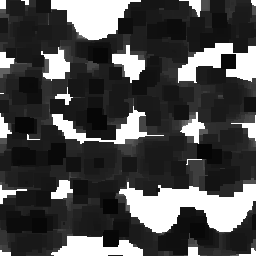
\includegraphics[width=.22\textwidth]{../screenshots/ism_splat_cropped} &
     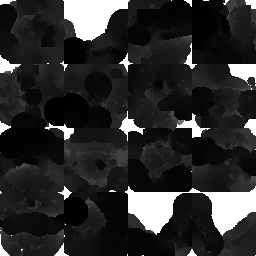
\includegraphics[width=.22\textwidth]{../screenshots/ism_single_pixel_cropped}
   \end{tabular}
   \caption{ISMs rendered using the splat renderer (left) and single-pixel renderer (right) with default settings. The single-pixel renderer performs interpolation between points, uses more points and doesn't let points ``bleed'' into neighboring ISMs, but takes more time.}
   \label{fig:results:isms}
 \end{figure}

 \Cref{fig:results:isms} shows a few ISMs rendered with the splat and single-pixel renderer. The imperfections do show, and not only through the low resolutions. The distortion of the surface silhouettes by the splat renderer or postprocessing contribute their part, making it hard to identify which part of the Crytek Sponza is shown.

 \begin{figure}[htb]
 \centering
   \begin{tabular}{@{}cc@{}}
     \includegraphics[width=.22\textwidth]{../screenshots/darkening_splat} &
     \includegraphics[width=.22\textwidth]{../screenshots/darkening_single_pixel}
   \end{tabular}
   \caption{Darkening caused by the splat renderer (left) compared to the single-pixel renderer (right). Note that there is no skylight rendered, which leads to an unnaturally dark upper part in the image even for the single-pixel renderer.}
   \label{fig:results:ismDarkening}
 \end{figure}

 Comparing the screenshots in \Cref{fig:results:ismDarkening}, it becomes apparent that the splat renderer causes visible darkening in the upper part of the image. The reason is likely that the point splats are always oriented towards the camera and do not take the point's normal into account when rendering, amplifying the usual aliasing artifacts of common shadow maps. As a result, any point size larger than one pixel causes surfaces that are not directly facing the camera appear nearer than they actually are when doing shadow lookups in the ISMs. A larger shadow bias could compensate for that but would introduce heavier light leaking. Another possibility would be to use the normal to calculate a point's depth per fragment at a potentially high performance cost.

 As the single-pixel renderer does not use splats, it does not have this problem. One could say it performs the per-fragment depth calculation implicitly during interpolation in the postprocessing phase.


 \begin{figure}[htb]
 \centering
   \begin{tabular}{@{}cc@{}}
     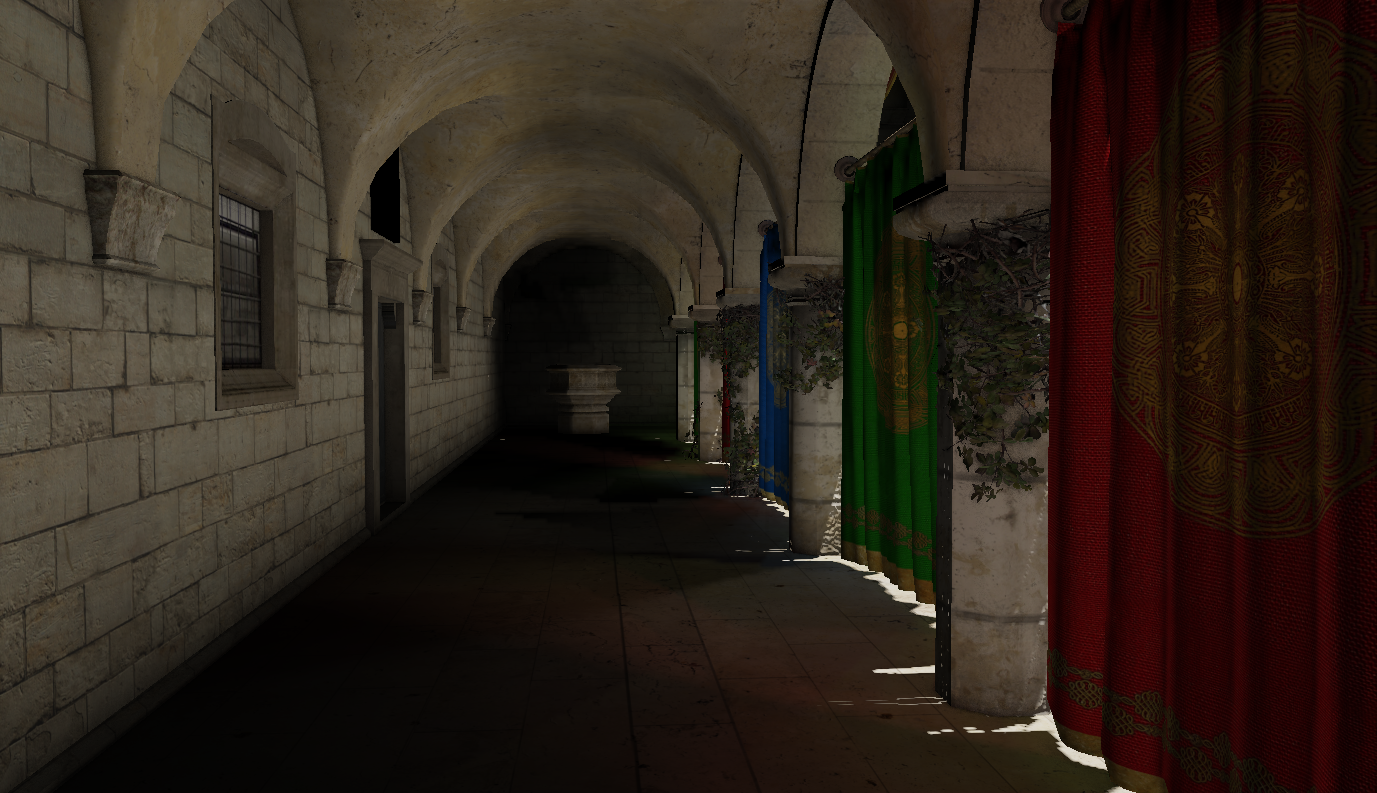
\includegraphics[width=.22\textwidth]{../screenshots/leaks_splat} &
     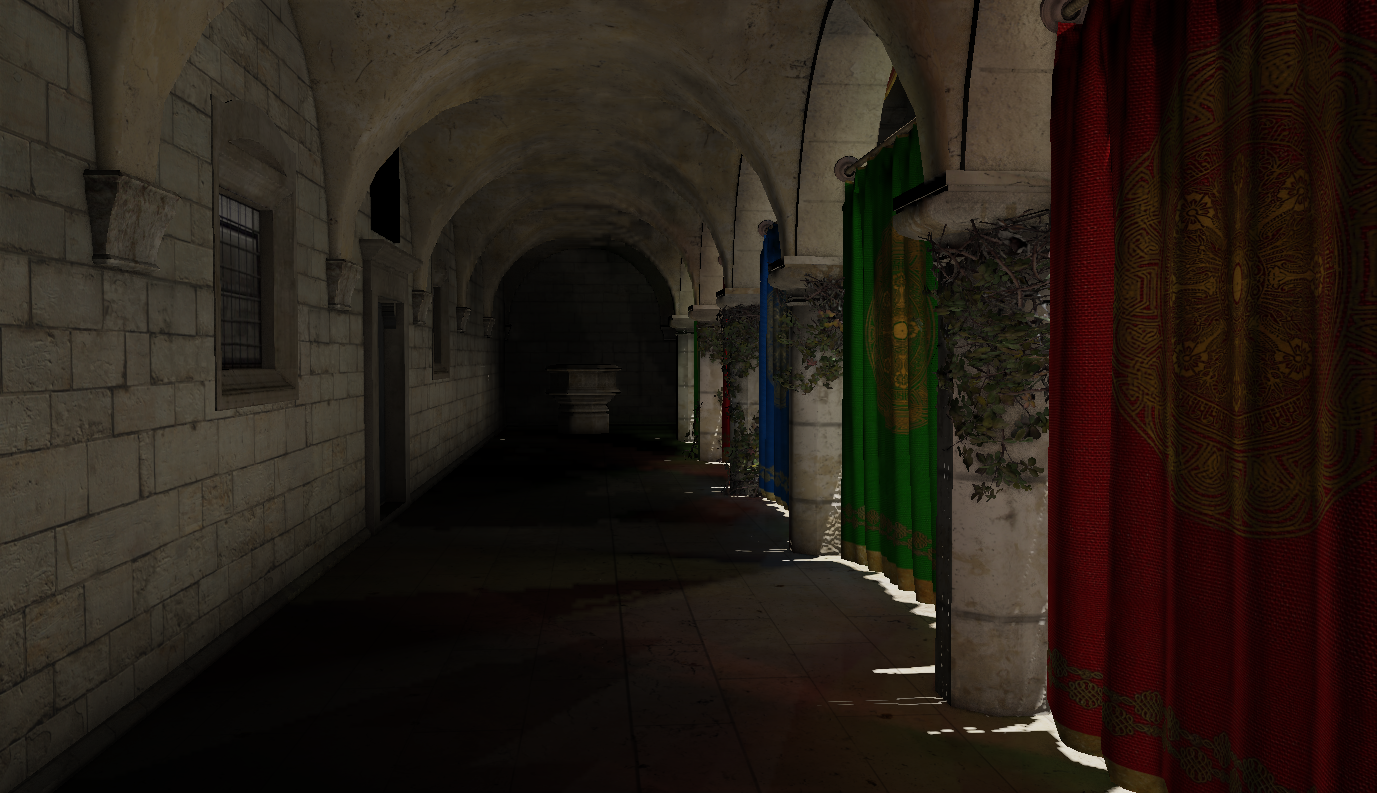
\includegraphics[width=.22\textwidth]{../screenshots/leaks_single_pixel}\\
     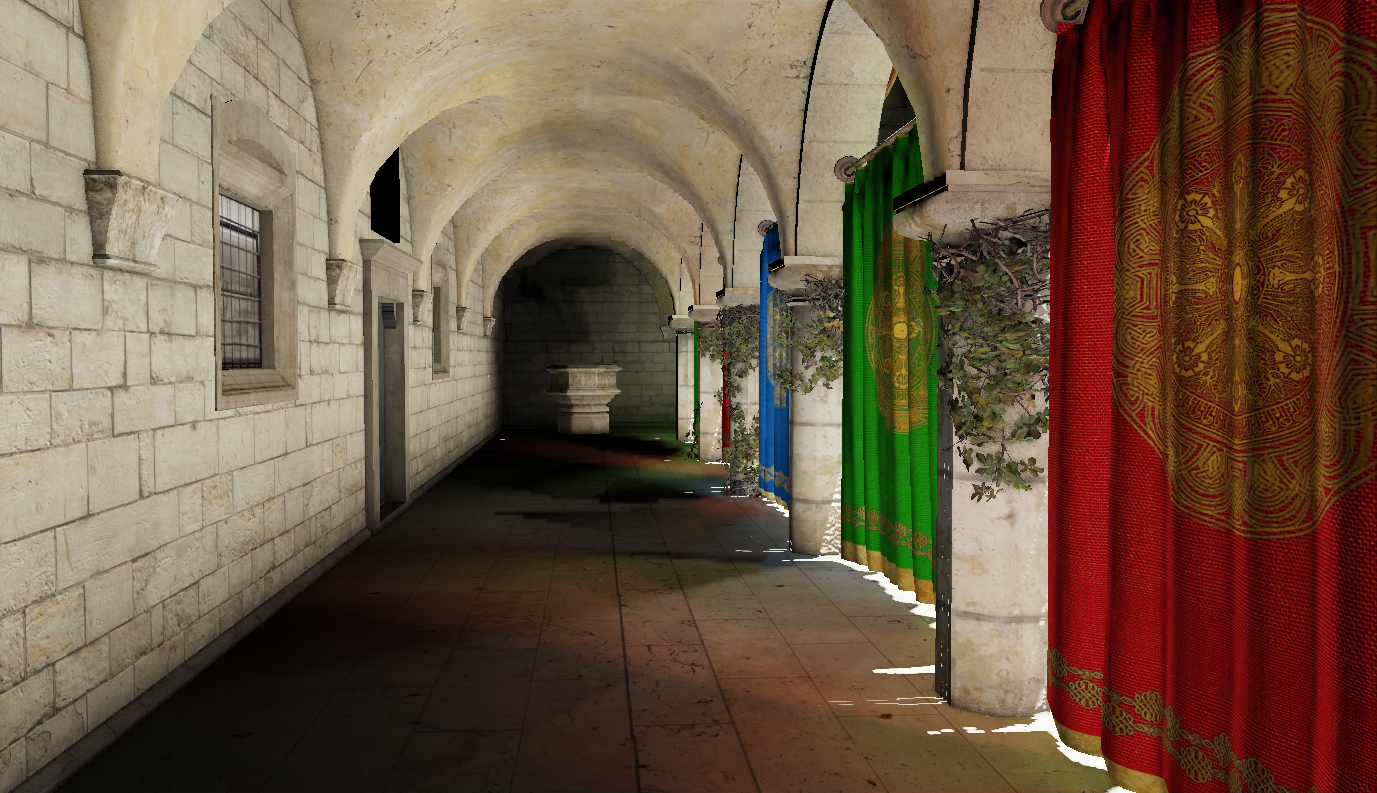
\includegraphics[width=.22\textwidth]{../screenshots/leaks_splat_exposure} &
     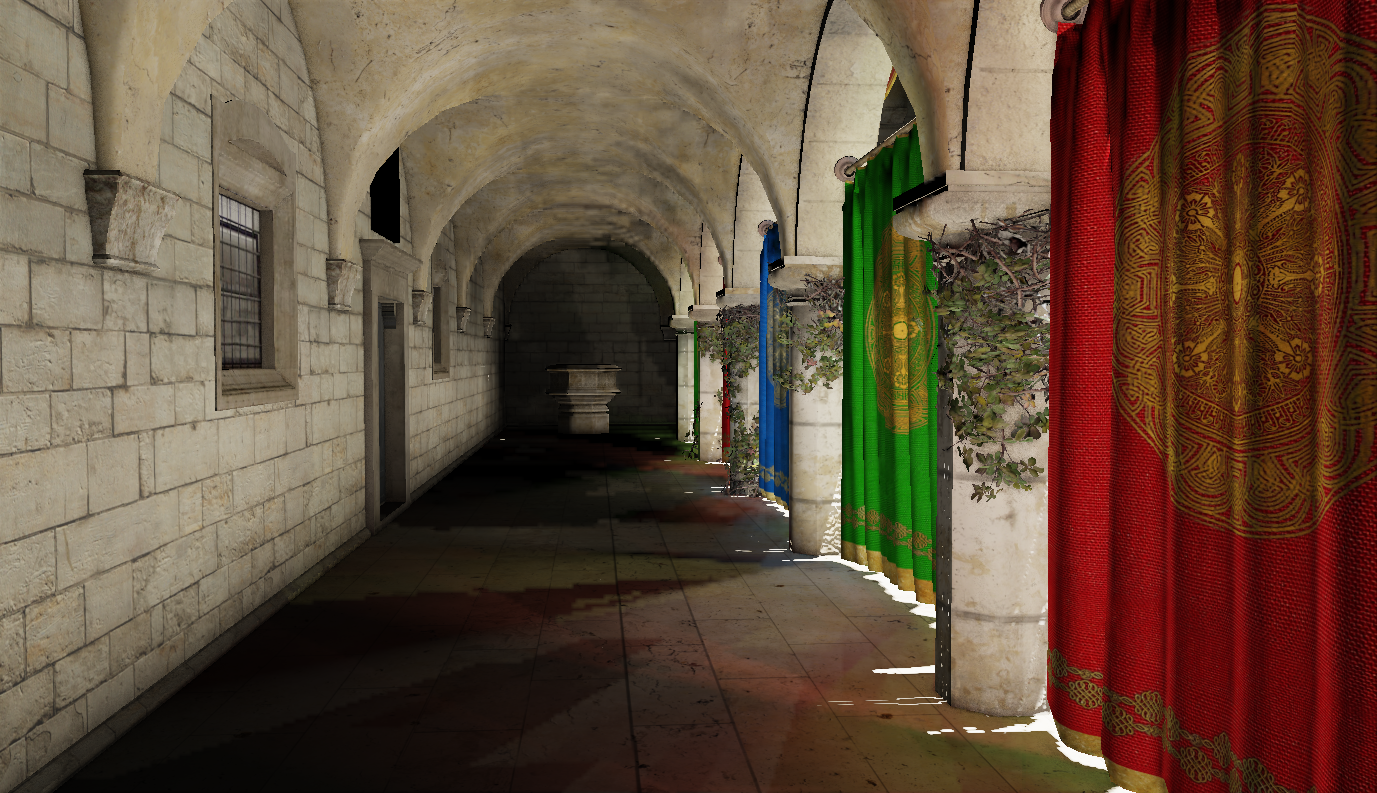
\includegraphics[width=.22\textwidth]{../screenshots/leaks_single_pixel_exposure}
   \end{tabular}
   \caption{Light leaks caused by the Imperfect Shadow Maps rendered with the splat renderer (left) and single-pixel renderer (right). VPLs from beneath the curtains leak light onto the wall and ceiling, while VPLs on the pillars and curtains light the floor. The renderings in the bottom row use a higher exposure for illustration. }
   \label{fig:results:leaks}
 \end{figure}


 \Cref{fig:results:leaks} shows a case the ISM technique has difficulties with. The image should be mostly dark or at least uniformly lit through the small gap below the curtains, but instead the wall and ceiling receive a lot of light and the floor displays several artifacts. The root cause is that the VPLs are placed right behind the curtains, so the occluding geometry, i.\,e., the curtain, is very near to the light source. Due to the randomness involved when selecting the point set for rendering the ISMs, it often happens that the points near to the light source are rendered into other ISMs, leaving a large hole behind. The single-pixel renderer copes a bit better than the splat renderer since it uses more points, but does not provide a satisfactory result either.



 \begin{figure}[htb]
 \centering
   \begin{tabular}{@{}cc@{}}
     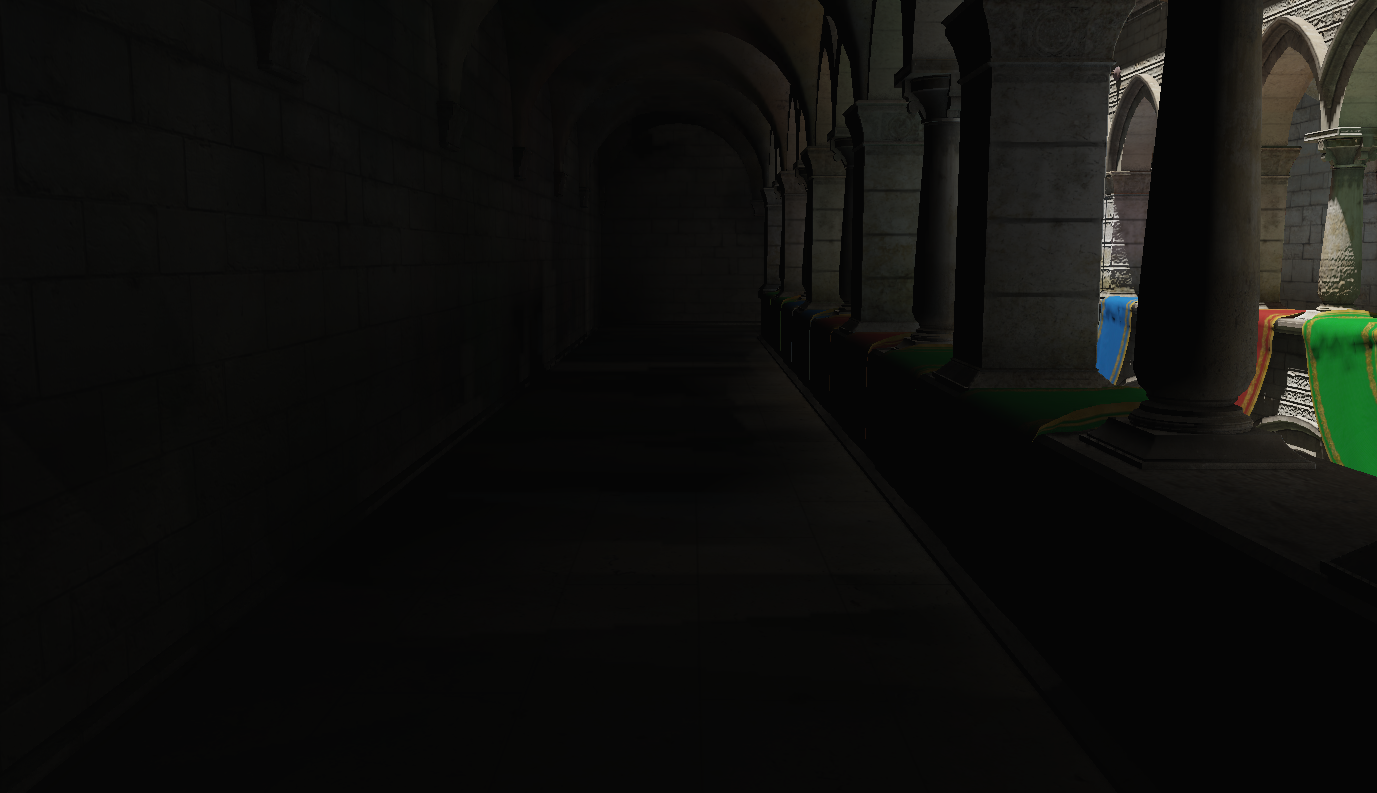
\includegraphics[width=.22\textwidth]{../screenshots/bias_splat} &
     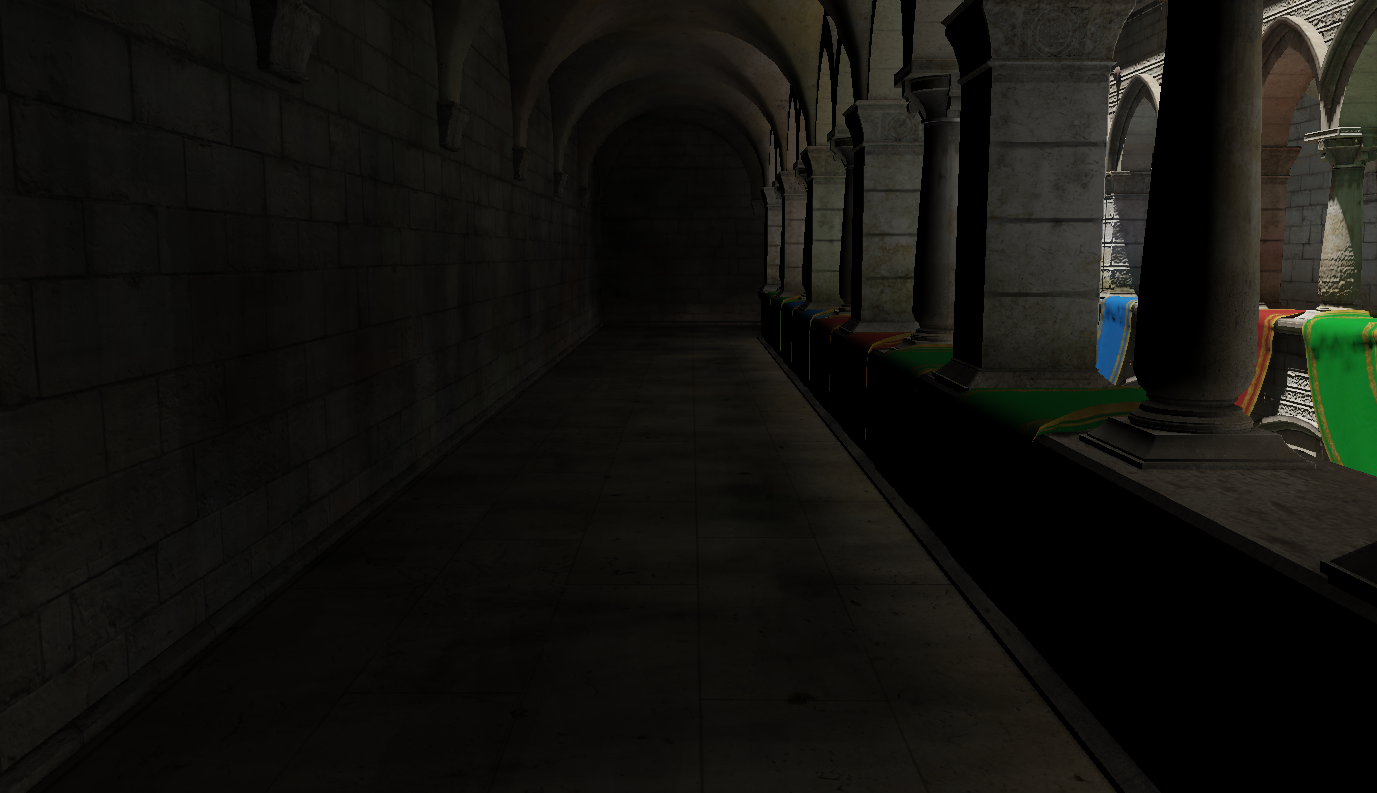
\includegraphics[width=.22\textwidth]{../screenshots/bias_single_pixel}\\
       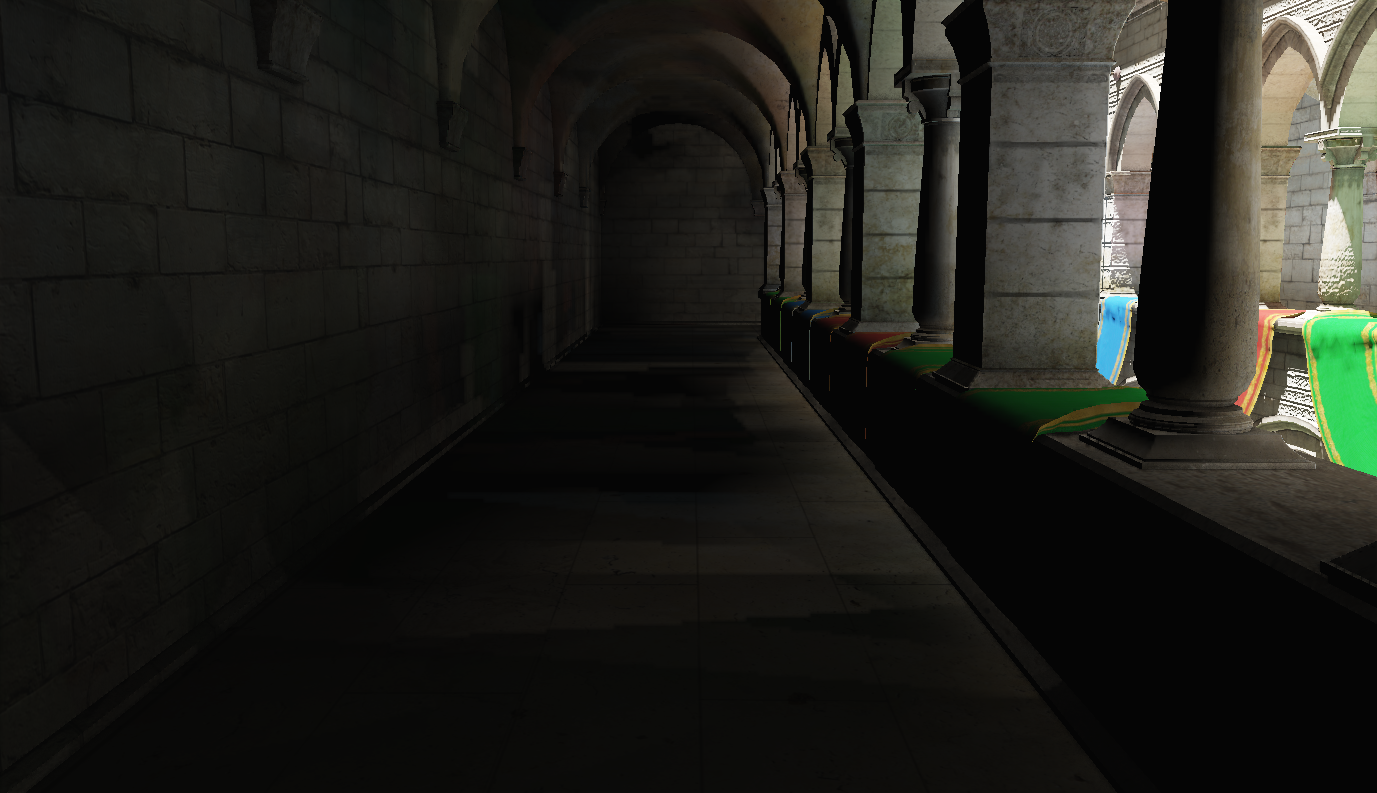
\includegraphics[width=.22\textwidth]{../screenshots/bias_splat_exposure} &
       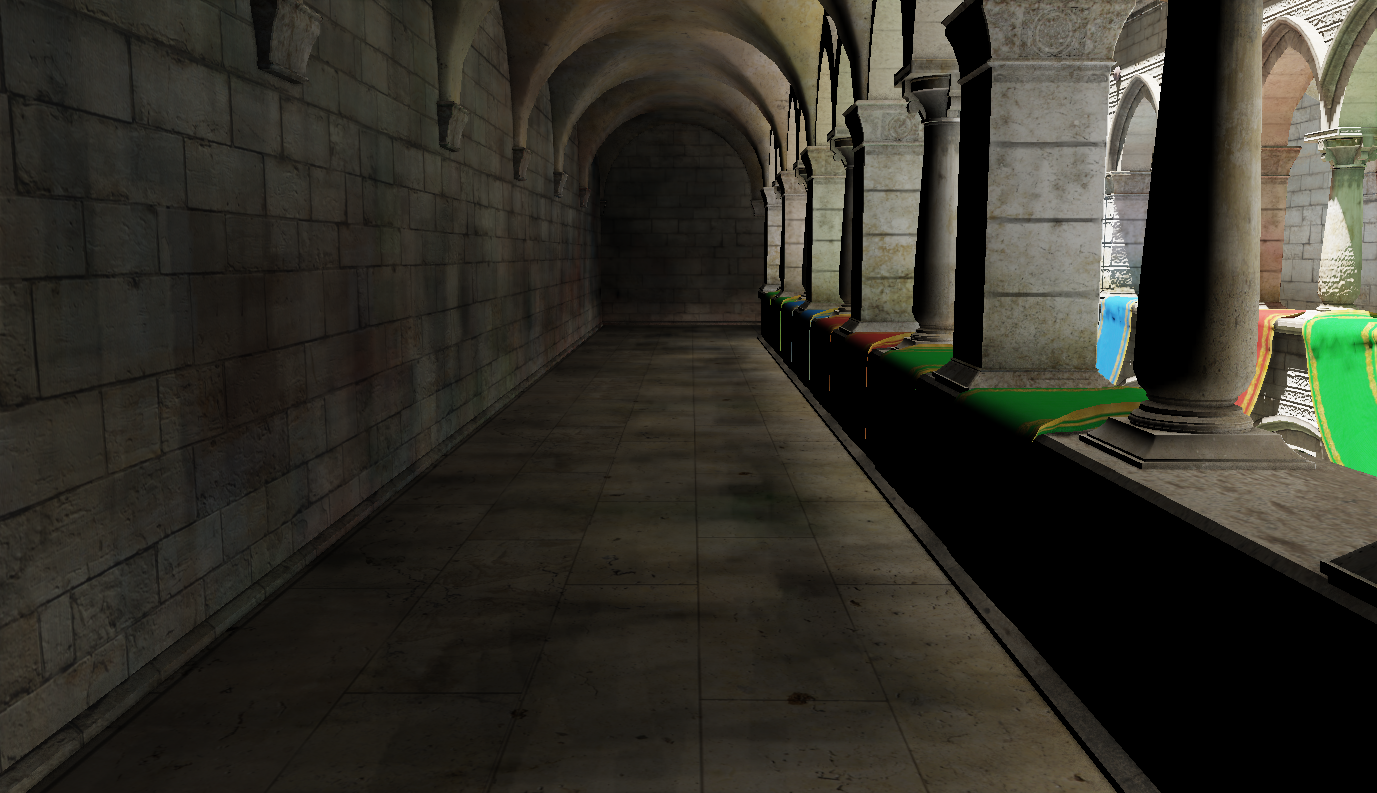
\includegraphics[width=.22\textwidth]{../screenshots/bias_single_pixel_exposure}
   \end{tabular}
   \caption{Light leaks caused by using a relatively large shadow bias with the purpose to hide artifacts of the ISMs. The screenshots to the left use the splat renderer, the right ones the single-pixel renderer. Bottom row uses a higher exposure.}
   \label{fig:results:bias}
 \end{figure}

 Our implementation hides some of the inaccuracies of the ISMs by using a relatively large shadow bias. The resulting light leaks are shown in \Cref{fig:results:bias}. While the splat renderer fares better here, it does so mainly by darkening the whole image since it uses rather large points. The single-pixel renderer on the other hand correctly lets light shine through the columns, but shows a very noisy result on the left wall.




 \subsection{Performance}
 \label{sec:results:performance}
  \vspace{0.1em}

 \begin{table}[h]
 \begin{center}
     \begin{tabulary}{0.475\textwidth}{| L | L | L | L |}
         \hline
         Splat Default Settings & Single-Pixel Default Settings & Splat with Single-Pixel Settings & Single-Pixel with Splat Settings \\ \hline
         3.4\,ms & 8.5\,ms & 38\,ms & 6.2\,ms \\
         \hline
     \end{tabulary}
     \caption{Timings of the ISM renderers with different settings.}
     \label{tab:results:ism_timings}
 \end{center}
 \end{table}
 \vspace{-0.5em}

 \Cref{tab:results:ism_timings} shows the time needed for rendering the ISMs with both renderers and different settings.

 Note that the comparison between the two renderers with default settings is not a fair one, since the single-pixel renderer uses more points and performs clamping per default. If the splat renderer is changed to behave similarly, it takes one additional millisecond for the clamping, and 33 additional milliseconds for using the same technique to collect VPLs as the single-pixel renderer does. There are several reasons for this heavy slowdown: First, we implemented this by emitting multiple vertices in the geometry shader, which is known to have poor performance on current GPUs. Second, the additional fillrate and overdraw became an issue when using too many points, a bottleneck that is unlikely to occur when using the single-pixel renderer. And third, while the single-pixel renderer uses shared memory to load the 16 VPLs once, the fragment shader of the splat renderer has no access to shared memory and has to load all 16 VPLs per invocation, creating high register pressure.

 Conversely, if the single-pixel renderer does not perform clamping, the push phase needs 0.3\,ms less (2.4\,ms to 2.1\,ms), and when it considers only one VPL per point, the point renderer uses 2.0\,ms less (2.9\,ms to 0.9\,ms).

 Since the technique implements no adaptivity, these numbers are independent from the viewport. They are however slightly affected by VPL placement, since it influences culling. In a second scenario, where the sunlight shines directly from above, all VPLs are placed on the floor facing up. As a result, much fewer points are culled during ISM rendering, resulting in slightly higher timings. The splat renderer needed an additional 0.7\,ms, whereas the single-pixel renderer needed only 0.2\,ms more.






 \subsection{Detailed Performance Measurements for the Single-Pixel Point Renderer}


% \setlength{\tabcolsep}{.16667em}
 \begin{table}[h]
 \tymin=22pt
 \tymax=61pt
 \begin{center}
     \begin{tabulary}{0.475\textwidth}{| L | L| L | L || L |} \hline
         Point Collection  & Point Rendering & Pull Phase & Push Phase & Total \\ \hline
         2.1\,ms & 3.0\,ms & 1.0\,ms & 2.4\,ms & 8.5\,ms \\ \hline
     \end{tabulary}
     \caption{Timing breakdown of the single-pixel point renderer.}
     \label{tab:results:timing_breakdown_single_pixel}
 \end{center}
 \end{table}
 \vspace{-0.5em}

 \begin{table}[h]
 \begin{center}
     \begin{tabulary}{0.475\textwidth}{| L | L  | L | L | L | L || L | L || L |}
         \hline
         PL 1 & PL 2 & PL > 2 & PS > 1 & PS 1 & PS 0 & PL T & PS T & T \\ \hline
         0.57 & 0.34 & 0.14 & 0.27 & 0.71 & 1.47 & 1.05 & 2.46 & 3.5\\
         \hline
     \end{tabulary}
     \caption{Timing breakdown of the pull (PL) and push (PS) phase, and total timings (T). The numbers of the individual steps indicate to which mipmap level they write, which is why the pull phase starts with 1 and the push phase has descending numbers. All timings are in milliseconds.}
     \label{tab:results:timing_breakdown_pull_push}
 \end{center}
 \end{table}
 \vspace{-0.5em}


 \Cref{tab:results:timing_breakdown_single_pixel} gives more detailed performance measurements of the single-pixel renderer, while \Cref{tab:results:timing_breakdown_pull_push} further breaks down the individual steps of the pull and push phase. The timings scale roughly as expected, since PL 3 and PS 2 (not separately listed in the table) are taking roughly 4 times longer than PL 2 and PS 1, respectively. However, the first and last step fall out of line. This is due to the reduced input data size (or output size, respectively), as explained in \Cref{sec:impl:pullPushPostprocessing}. Also note how the push phase does take roughly the time of the pull phase if it were not for the last phase, where it writes to the full 2048\,px\textsuperscript{2} of miplevel zero, whereas the first pull phase only writes to the miplevel one with 1024\,px\textsuperscript{2}.



 % show this is bandwidth bound. calculation how much memory is read and written, vs bandwidth of GTX 980.
 %     - roughly 110MB read and written, that's 1.2ms.
 %     - 16MB of that unnecessarily because of the 2nd layer of input texture
 %     - By parallel reduction juju reduced by 22MB or 0.2ms.
 %     - with more juju, maybe brought down to actually that time, except for the arithmetic stuff of course...


 \subsection{Memory Usage}

 The point splat renderer uses no more memory than the ISM texture itself requires, which is 8\,MB for a 2048\,px\textsuperscript{2} 16-bit depth buffer.

 The single-pixel renderer uses additional memory. The buffer for storing points is implemented as four-channel 32-bit float texture, with the position in the first three channels, and the radius (8 bit) and normal (24 bit, see \cite{Cigolle:2014:NormalPacking}) in the fourth channel. With a maximum point count of 2048 per ISM, this buffer uses 32\,MB.
 The additional textures used are the render target of the single-pixel renderer (single-channel 2048x2048x2\,px, 32-bit integer, 32\,MB), the mipmap levels used by the pull-push algorithm (two channels, 32-bit, approx. 11\,MB) and the final ISM (same as used by the splat renderer, uses 8MB).

 Added together, the single-pixel renderer uses a total of 83\,MB, likely with room for optimization left.



 \subsection{Comparison of the Splat and Single-Pixel Renderer}

 The single-pixel renderer provides numerous advantages over the splat renderer. Using a compute shader to render the points lifts the restrictions of the fixed-function pipeline and e.\,g.\ enables rendering each point into multiple ISMs without large performance losses. Quality-wise, it can reproduce surfaces more accurately by correctly interpolating between points.

 The drawbacks obviously include the additional rendering time and memory. Besides, the added complexity should not be underestimated. Specifically, we found it hard to fine-tune the pull-push algorithm to give us satisfactory results, especially in the face of the low resolutions of ISMs and the limited data available for reconstruction after selecting a random and sparse set of points.





 \section{Discussion}


 Imperfect Shadow Maps have several deficits, some of which are inherent to the technique and difficult to solve, others are specific to the implementation choices and tradeoffs in our implementation and might be easier to overcome.

 First, ISMs reduce the scene's geometry to points. At the resolution that is achievable in a real-time budget, this is already a stark approximation that loses a lot of accuracy.

 Second, because a sparse set of points is used for each ISM, each point must be enlarged to accomodate for the neighboring points that are likely missing in the chosen ISM. For instance, if an area is represented by a thousand points and only one tenth of all points is used for each ISM, each remaining point's area must be enlarged by a factor of ten to result in an equally large area in the rendered output. Of course, this approach leads to deformed geometry since points at the edges of the area get enlarged as well, growing over the borders of the original geometry.

 Third, there are also numerical issues. For instance, both the splatting and postprocessing approaches ignore the distortion caused by the projection, and thus might render even simple surfaces incorrectly. This contributes to the necessity of using a relatively large shadow bias. This can likely be solved, albeit at the cost of additional complexity.

 Fourth, and this is in our view the most important shortcoming, ISMs handle geometry in the vicinity to VPLs badly as can be seen in \Cref{fig:results:leaks}. To sufficiently approximate such surfaces when rendering ISMs, one would need to greatly increase the number of points created near VPLs, possibly in addition to stepping away from using a fully random approach for point selection and select a specific point set for each ISM depending on the VPLs location.

 As for most global illumination algorithms, a massive improvement would be to differentiate between large-scale scene geometry that is important for diffuse light bounces, and smaller geometry of lesser importance. While the latter can possibly be ignored altogether with only minor losses in quality, the shape of large-scale geometry is all the more important to preserve (relatively) precisely.



\section{Conclusion}

In this paper, we have presented extensions to the Imperfect Shadow Map algorithm that allow greater accuracy at the cost of performance and memory. Compared to the original algorithm, our extensions make it scale better with the number of points, a determinant for the quality of the shadow map, and reconstruct surfaces from the available points more accurately.

However, we do think that there is a rather low upper bound in quality that is achievable with the approach of randomly selecting points, especially in geometrically complex scenes. To mitigate this, the selection of points needs to be heavily improved or alternate methods of rendering masses of shadow maps need to be investigated.
